\documentclass[UKenglish]{scrreprt}

\RequirePackage[numbers, round]{natbib}
\RequirePackage[utf8]{inputenc}              % Direkte Eingabe von ä usw.
\RequirePackage[T1]{fontenc}                 % Font Kodierung für die Ausgabe        
\RequirePackage{babel}                       % Verschiedenste sprach-spezifische Extras
\RequirePackage[autostyle=true]{csquotes}    % Intelligente Anführungszeichen
\RequirePackage{graphicx}                    % zum Bilder einbinden
\RequirePackage[]{amssymb}                   %
\RequirePackage{amsmath}                     %Mathekram
\RequirePackage{physics}                     %Für Einheiten und so
\RequirePackage{hyperref}                    %
\RequirePackage[all]{hypcap}                 %
\usepackage{siunitx}
\usepackage{longtable}
\usepackage{booktabs}
\RequirePackage{newtxmath}                   % Schönere Schriftart
\RequirePackage{newtxtext}                   % Schönere Schriftart    
\KOMAoptions{fontsize=11pt, paper=a4}        % Schriftgröße und Papierformat setzen
\KOMAoptions{DIV=11}                         % Parameter mit dem man den Seitenrand ändern kann
\KOMAoptions{listof=totoc}                   % Abbildungs- und Tabellenverzeichnis im Inhaltverzeichnis  aufzuführen


\title{Where should I go? Finding the optimal neighborhood in Bonn to move to from Munich}
\subtitle{IBM Applied Data Science Capstone Project}
\author{Laila Linke}
\date{\today}

\begin{document}

\maketitle

\pagenumbering{roman}

\chapter*{Executive summary}

\paragraph{Key question:}In this report, we answer the following key question: \emph{Which neighborhoods in the German city Bonn are most similar to the cite center of Munich?} This question is relevant for people who plan to move from Munich to Bonn and want to choose their new neighborhood to have similar stores, amenities, and restaurants as their current living place. 

\paragraph{Data \& Methodology:} We tackle the key question with data on the location and category of venues from Foursquare. We combine this data with publicly available data from Bonn's city administration, which contains the shapes and coordinates of Bonns neighborhoods. Using this data, we find the most common venue categories for each neighborhood in Bonn and compare these to the most common venues near the University of Munich. We also cluster similar areas in Bonn using the k-means clustering algorithm and find the neighborhood cluster in Bonn closest to Munich. 

\paragraph{Results:}Our results are
\begin{itemize}
	\item The neighborhoods most similar to the city centre of Munich are \emph{Südstadt} and \emph{Bonn-Zentrum}.
	\item The neighborhood cluster most similar to Munich consists primarily of areas at the river Rhine.
	\item The neighborhoods \emph{Ückesdorf} \emph{Holzlar} and \emph{Geislar} are the most dissimilar to Munich
\end{itemize}
%
\paragraph{Recommendations:}Based on these results, we recommend a person moving from Munich to Bonn to \emph{move preferably to Südstadt} and to \emph{avoid moving to Ückesdorf}.


\tableofcontents
\clearpage

\pagenumbering{arabic}


\chapter{Introduction}
\section{Background}
Bonn and Munich are two German cities that, at first glance, are quite dissimilar. Munich is a big metropolis with \num{1485671} inhabitants\footnote{as of 30th September 2020 }\cite{muenchen}, while Bonn has only \num{329673} \footnote{as of 30th September 2019}
\cite{bonn}. Due to the different population numbers, it is plausible that different kinds of restaurants, stores, and leisure amenities exist in those two cities. For example, based on its smaller population, we expect Bonn to have less variety in international cuisine. 

However, this is not necessarily the case for all of Bonn. Bonn consists of 51 different neighborhoods, whose structure and population vary. For example, the area near the Rhine contains international embassies and offices of the United Nations. Therefore, these areas to be more global and have more amenities than the \enquote{average} neighborhood in Bonn.

For a person moving to Bonn, these differences between the neighborhoods pose a problem: Which neighborhood should they choose so that the restaurants, stores, and other venues near them fulfill their expectations? This is precisely the problem we are studying in this report.

\section{Problem}
We are investigating the following problem. A person currently living in the \emph{Kaulbachstraße} next to the main building of Munich University is planning a move from their current home to Bonn. They enjoy the amenities and variety of venues in their current neighborhood and therefore want to move to an area with a similar structure. Our goal is to recommend the neighborhoods best suited to this person. 

\section{Proposed methodology and structure of this report}

To solve the problem, we study the venues in each of Bonns neighborhoods and compare them to venues near the current home in Munich. We find the most common categories of venues per neighborhood and use them to define the similarity between each of Bonn's neighborhoods and Munich. Based on this similarity, we recommend which area the person should move to, and which they should avoid.

Our analysis consists of three parts. We qualitatively explore the data by finding the most common venue categories per neighborhood in the first part. In the second part, we quantify each neighborhood's similarity with the Munich area and find the single most similar neighborhood. In the third part, we group comparable neighborhoods into clusters and find the cluster most resembling Munich.

This report is structured as follows: In Section \ref{sec:Data} we introduce the data sets we used.  Section \ref{sec:Analysis} details our analysis of the data. This analysis includes an exploratory assessment of the most common venue categories per neighborhood (Sect.~\ref{sec:Analysis: Exploratory}), the determination of the similarity of each neighborhood in Bonn to Munich (Sect.~\ref{sec:Analysis:Neighborhood}), and the ranking of neighborhood clusters according to their similarity to Munich (Sect.~\ref{sec:Analysis:Cluster}). The results of our analysis are presented in Sect.~\ref{sec:Results}. We discuss them and give our final recommendations in Sect.~\ref{sec:Discussion}. Sect.~\ref{sec:Conclusion} summarizes this report and gives some directions for future exploration.

The full code for our analysis is available as a \href{https://github.com/llinke1/Coursera\_Capstone/blob/main/CapstoneProject\_OptimalNeighborhoodBonn.ipynb}{Jupyter Notebook}.

\chapter{Data}
\label{sec:Data}

\section{Used Datasets and -sources}
In this analysis, we require data on the location of Bonn's neighborhoods. We also need the location and category of restaurants, stores, and other venues in Bonn and near the current home in Munich. We describe our two data sets in the following.

\subsection{Location and center of Bonn's neighborhoods}
We use the location and borders of Bonn's neighborhoods provided by the city administration on their open data platform \footnote{\href{https://opendata.bonn.de/dataset/fl\%C3\%A4chen-der-ortsteile}{https://opendata.bonn.de/dataset/fl\%C3\%A4chen-der-ortsteile}}\cite{Ortsteile}. This data is available as a GeoJSON file and contains the name, ID and polygon shape of each of the 51 neighborhoods (in German: \enquote{Stadtteile}), as well as their respective city district and district ID.
The data was first published on 11th February 2015 and is updated daily. It is available publicly under a Creative Commons CC Zero License, meaning that 
it is in the Public Domain and can be freely used and shared for any purpose.

We access the data with the python package \verb|geopandas|\footnote{\href{https://geopandas.org/}{https://geopandas.org/}} and read it into a data frame. We also visualize the location of Bonn's neighborhoods, using the \verb|folium| package \footnote{\href{https://python-visualization.github.io/folium/}{https://python-visualization.github.io/folium/}}. The resulting map is shown in Fig.~\ref{fig: map neighborhoods}.

\begin{figure}[htbp]
	\centering
	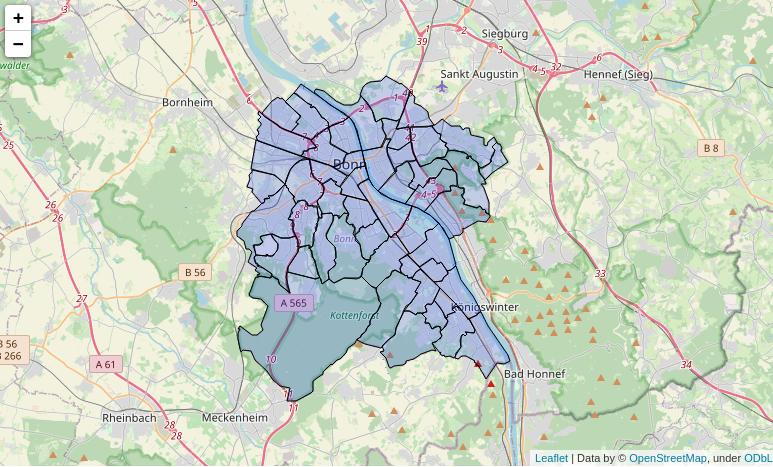
\includegraphics[width=\textwidth]{Figs/Map_Neighborhoods.png}
	\caption{Map of Bonn with neighborhoods overlayed in blue and centres of neighborhoods marked by blue circles. Location and shape of neighborhoods is from \cite{Ortsteile}, the map of Bonn was created with \texttt{folium}.}
	\label{fig:map neighborhoods}
\end{figure}

To simplify our analysis, we drop the columns describing the neighborhood ID, the district name, and the district ID from this data frame, as these are not related to our analysis. We also find the center of each neighborhood using the \verb|centroid| method of \verb|geopandas| and add the centers' longitude and latitude to the data frame as new columns. Table~\ref{tab: neighborhoods} shows the first five rows of the data frame of Bonn's neighborhoods used in the following analysis.

\begin{table}
	\caption[First five rows of neighborhood data]{First five rows of \texttt{neighborhoods} data frame, containing the name, shape, and center coordinates of Bonn's neighborhoods. Data from \cite{Ortsteile}}
	\label{tab:neighborhoods}
	\begin{tabular}{lllrr}
		\toprule
		{} &          name &                                           geometry &  longitude &   latitude \\
		\midrule
		0 &      Auerberg &  POLYGON ((7.06486 50.75323, 7.06502 50.75339, ... &   7.070968 &  50.755913 \\
		1 &  Bonn-Castell &  POLYGON ((7.09779 50.75559, 7.09781 50.75560, ... &   7.097325 &  50.747996 \\
		2 &  Bonn-Zentrum &  POLYGON ((7.10191 50.73247, 7.10163 50.73225, ... &   7.101694 &  50.736540 \\
		3 &     Buschdorf &  POLYGON ((7.06502 50.75339, 7.06486 50.75323, ... &   7.053905 &  50.757436 \\
		4 &    Dottendorf &  POLYGON ((7.10961 50.70893, 7.10961 50.70890, ... &   7.115320 &  50.703584 \\
		\bottomrule
	\end{tabular}
\end{table}


\subsection{Location and categories of venues}
To obtain the location and categories close to the Munich address and in each neighborhood in Bonn, we use Foursquare. 
Foursquare is a search and discovery mobile app that provides users with the opportunity to find new venues close to them, recommend and review visited venues and \enquote{check-in} at their favorite places. Due to the app's popularity, Foursquare has obtained a large dataset of the location, category, and rating of venues like restaurants, stores, and leisure amenities all over the world. This dataset is accessible via an Application Programm Interface (API), which we use for our analysis.
Using the Foursquare API and data commercially requires a paid subscription. However, here we are only considering personal use, which is free. 

We use the API to obtain the name, location, and category of each venue listed on Foursquare within 500 m of the center of each of Bonn's neighborhoods and the Kaulbachstraße in Munich. From the API, we obtain 433 venues in Bonn, most of which are supermarkets, and 38 in Munich, most of which are cafés. The first five rows of the data frame containing the venues in Bonn are shown in Table~\ref{tab:venues_Bonn}, while the first five rows of the data frame containing the venues in Munich are shown in Table~\ref{tab:venues_Munich}.

\begin{table}
	\caption{First five rows of \texttt{venues\_Bonn} data frame, containing the neighborhood, neighborhood centre coordinates, venue name, venue coordinates and venue category of venues in Bonn.}
	\label{tab:venues_Bonn}
\begin{tabular}{lp{1.5cm}p{2.2cm}p{2.2cm}p{1.5cm}p{1.5cm}p{1.5cm}p{1.5cm}}
	\toprule
	{} & Neighbour-hood &  neighborhood Latitude &  neighborhood Longitude &                   Venue &  Venue Latitude &  Venue Longi-tude &  Venue Category \\
	\midrule
	0 &     Auerberg &              50.755913 &                7.070968 &  H Kopenhagener Strasse &       50.757418 &         7.071644 &    Tram Station \\
	1 &     Auerberg &              50.755913 &                7.070968 &                    REWE &       50.755647 &         7.076839 &     Supermarket \\
	2 &     Auerberg &              50.755913 &                7.070968 &      H Auerberger Mitte &       50.755102 &         7.076088 &    Tram Station \\
	3 &     Auerberg &              50.755913 &                7.070968 &                   PENNY &       50.756300 &         7.076302 &     Supermarket \\
	4 &     Auerberg &              50.755913 &                7.070968 &         Packstation 116 &       50.752412 &         7.073921 &  Shipping Store \\
	\bottomrule
\end{tabular}
\end{table}


\begin{table}
	\caption{First five rows of \texttt{venues\_Munich} data frame, containing the neighborhood, neighborhood centre coordinates, venue name, venue coordinates and ven¸ue category of venues in Bonn.}
	\label{tab:venues_Munich}
\begin{tabular}{lp{1.5cm}p{2.2cm}p{2.2cm}p{1.5cm}p{1.5cm}p{1.5cm}p{1.5cm}}
	\toprule
	{} & Neighbour-hood & neighborhood Latitude &  neighborhood Longitude &                     Venue &  Venue Latitude &  Venue Longitude & Venue Category \\
	\midrule
	0 &       Munich &               48.15113 &                11.58415 &                  Dinatale &       48.150196 &        11.583001 &           Café \\
	1 &       Munich &               48.15113 &                11.58415 &  Geschwister-Scholl-Platz &       48.150850 &        11.581383 &          Plaza \\
	2 &       Munich &               48.15113 &                11.58415 &               Koenigin 43 &       48.150173 &        11.584367 &           Café \\
	3 &       Munich &               48.15113 &                11.58415 &               Milchhaeusl &       48.149882 &        11.585483 &    Beer Garden \\
	4 &       Munich &               48.15113 &                11.58415 &  DELI STAR Bagel \& Coffee &       48.150024 &        11.583972 &     Bagel Shop \\
	\bottomrule
\end{tabular}
\end{table}

To visually inspect the data, we display the venues and the neighborhood centers in Bonn in Fig \ref{fig: map venues_bonn}. This inspection reveals four neighborhoods, which do not have any listed venues (Röttgen, Schweinheim, Heiderhof, and Hardthöhe). Our analysis, therefore, cannot apply to these neighborhoods, and we drop their corresponding rows.

\begin{figure}[htbp]
	\centering
	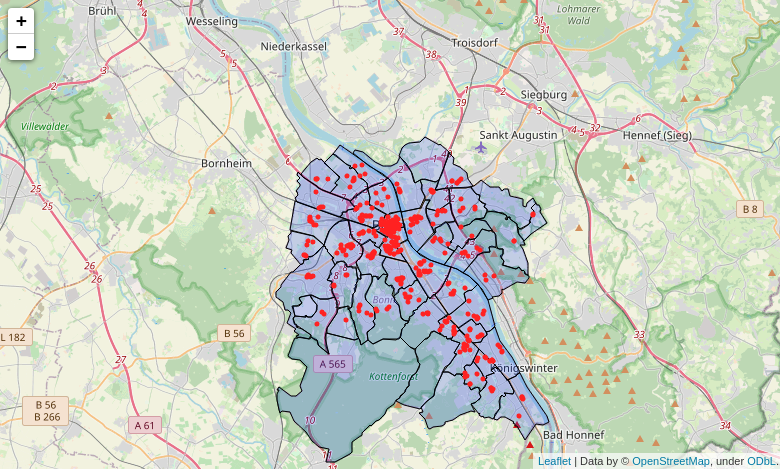
\includegraphics[width=\textwidth]{Figs/Map_Bonn_venues.png}
	\caption{Map of venues in Bonn (red circles) around neighborhoods centers (blue circles).}
	\label{fig:map venues_bonn}
\end{figure}

 
\chapter{Analysis}
\label{sec:Analysis}
Our analysis consists of three parts. In the first part, we qualitatively explore the data by finding the most common venue categories per neighborhood. In the second part, we quantify each neighborhood's similarity with the Munich area and find the single most similar neighborhood. In the third part, we group comparable neighborhoods into clusters and find the cluster of neighborhoods most similar to Munich.
\section{Exploratory Data Analysis}
\label{sec:Analysis: Exploratory}
In our exploratory analysis, we find the most common venue categories per neighborhood. For this, we first calculate the fraction of each venue category per neighborhood. The fraction of the venue category $i$ per neighborhood $j$ is given by
\begin{equation}
	f_{ij}=\frac{N_{ij}}{\sum_k N_{kj}}\;,
\end{equation} 
where $N_{ij}$ is the number of venues of category $i$ in neighborhood $j$, and the sum goes over all different venue categories. The higher this fraction, the more venues of a specific category are in a neighborhood.

We sort the venue categories by their fraction for each neighborhood and the Munich area and find the three most common categories.

\section{Determination of most similar neighborhood}
\label{sec:Analysis:Neighborhood}
To determine the most similar neighborhood to Munich, we define the \emph{dissimilarity} $d_{ij}$ of two areas $i$ and $j$ as
\begin{equation}
	d_{ij}=\sum_{k} (f_{ki}-f_{kj})^2\;,
\end{equation}
where the sum goes over all possible venue categories and $f_{ki}$ is the fraction of venues of category $k$ in neighborhood $i$.
The higher $d_{ij}$, the more dissimilar are $i$ and $j$. The dissimilarity corresponds to the Euclidean distance between two data points in the space spanned by the $f_{ij}$ features.

We also define the \emph{similarity} $s_{ij}$ as 
\begin{equation}
	s_{ij}=-\log_{10}(d_{ij})\;.
\end{equation}
This quantity becomes infinitely large, if two neighborhoods have exactly the same fraction of venues per category. A larger similarity index therefore indicates a closer resemblance of two neighborhoods.

We calculate the dissimilarity and the similarity index of each neighborhood compared to the Munich area. According to the $s_{ij}$, we rank the neighborhoods, find the one most resembling Munich, and visualize our results on a map. 

\section{Determination of most similar neighborhood cluster}
\label{sec:Analysis:Cluster}
Lastly, we group comparable neighborhoods into clusters and rank the clusters according to their similarity to Munich. To find the clusters, we employ a k-means algorithm.

The k-means algorithm works as follows. First, $k$ randomly chosen positions in the feature space (in our case: fraction $f_{ij}$ of each venue category $i$ in neighborhood $j$) are assigned as \emph{cluster centers}. Second, each data point (in our case: each neighborhood) is assigned to the cluster center to which it has the smallest Euclidean distance. Third, new cluster centers are computed as the centroids of each cluster. The data points are then reassigned to the newest closest cluster center. These steps continue iteratively until (and if) the algorithm converges.

A crucial choice for this algorithm is the number $k$ of clusters. To find the optimal value of $k$, we try out values of $k$ between 2 and 20 and compute the *inertia* for these values. The inertia is the sum of the squared Euclidean distance of each neighborhood to its cluster center. Plotting the inertia against $k$ (so-called Elbow plot) can give insight into the correct choice for $k$. 

Our \enquote{Elbow} plot is shown in Fig.~\ref{fig:ellbow}. It shows that the inertia decreases with increasing $k$. However, this decrease is not uniform. It is fast in the beginning, but for larger $k$ the decrease is slower. The optimal $k$ is at the transition between fast and slow inertia decrease. 

\begin{figure}
	\centering
	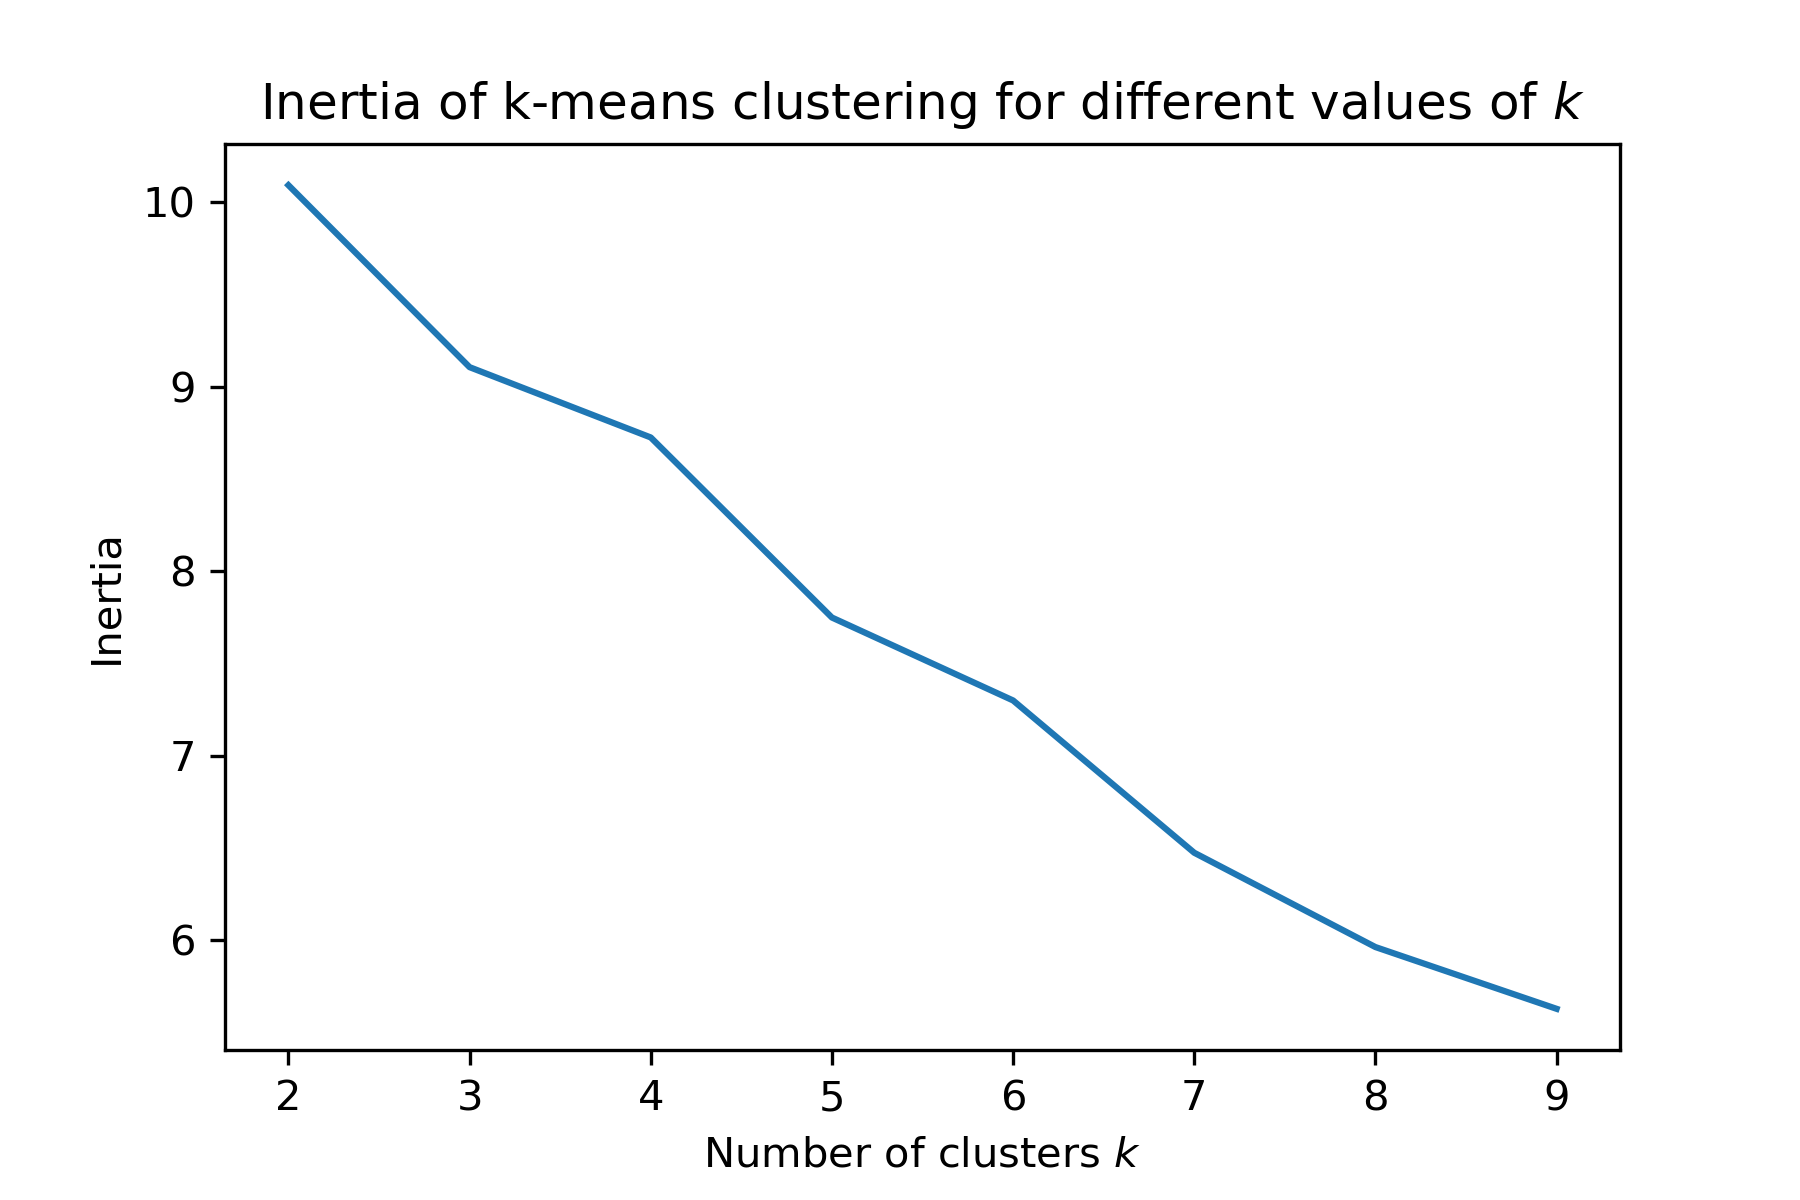
\includegraphics[width=0.7\linewidth]{Figs/Ellbowplot}
	\caption{Inertia of k-means clustering for different numbers $k$ of clusters. The inertia decreases with $k$. the transition between a strong and weak decrease gives the optimal choice for $k$, in our case $k=5$.}
	\label{fig:ellbow}
\end{figure}


Here, this transition is not obvious. However, we think that a $k$ of 5 is a reasonable guess for the transition, based on the above plot. Therefore we choose $k=5$, do a k-means clustering and assign each neighborhood a cluster label. Then, we calculate the dissimilarity and similarity index of each neighborhood cluster's centers and rank the neighborhoods based on their similarity to Munich.

\chapter{Results}
\label{sec:Results}

\section{Exploratory Data Analysis}
Based on each venue category's fraction, we find that the three most common venue categories in the Munich area are cafés, bars, and Italian restaurants. The most common venue types for the Bonn neighborhoods are listed in Table~\ref{tab:most_common_venues}.

\begin{table}
	\small
	\caption{Three most common venue categories per neighborhood in Bonn}
	\label{tab:most_common_venues}
\begin{longtable}{ll}
	\toprule
	Neighborhood &                                 Most common venues \\
	\midrule
	Alt-Godesberg                       &    Drugstore, Clothing Store, Italian Restaurant \\
	Auerberg                            &  Supermarket, Tram Station, Furniture / Home Supply Store \\
	Beuel-Mitte                         &                Ice Cream Shop, Café, Supermarket \\
	Beuel-Ost                           &                 Theater, Restaurant, Pizza Place \\
	Bonn-Castell                        &              Bus Stop, Hotel, Athletics \& Sports \\
	Bonn-Zentrum                        &                    Plaza, Bar, German Restaurant \\
	Brüser Berg                         &           Recreation Center, Supermarket, Garden \\
	Buschdorf                           &                    Gym, Soccer Field, Playground \\
	Dottendorf                          &  Supermarket, Spanish Restaurant, Italian Restaurant \\
	Dransdorf                           &             Supermarket, Drugstore, Tram Station \\
	Duisdorf                            &     Greek Restaurant, Gym, Vietnamese Restaurant \\
	Endenich                            &                 Theater, Plaza, Insurance Office \\
	Friesdorf                           &                Supermarket, Pool, Farmers Market \\
	Geislar                             &         Electronics Store, Wine Bar, Flea Market \\
	Godesberg-Nord                      &  Supermarket, Spanish Restaurant, Discount Store \\
	Godesberg-Villenviertel             &      Hotel, Food Truck, Mediterranean Restaurant \\
	Graurheindorf                       &       Spanish Restaurant, Bed \& Breakfast, River \\
	Gronau                              &                    Café, Restaurant, Art Gallery \\
	Hochkreuz                           &       Baseball Stadium, Asian Restaurant, Lawyer \\
	Hoholz                              &            Italian Restaurant, Butcher, Wine Bar \\
	Holtorf                             &                    Rest Area, Pharmacy, Wine Bar \\
	Holzlar                             &       Bus Stop, Wine Bar, Furniture / Home Store \\
	Ippendorf                           &             Soccer Field, Drugstore, Supermarket \\
	Kessenich                           &          Bakery, Italian Restaurant, Pizza Place \\
	Küdinghoven                         &             Scenic Lookout, Brewery, Fish Market \\
	Lannesdorf                          &               Ice Cream Shop, Plaza, Supermarket \\
	Lengsdorf                           &   Drugstore, Gluten-free Restaurant, Supermarket \\
	Lessenich/Meßdorf                   &                          Pub, Concert Hall, Farm \\
	Limperich                           &                  Tram Station, Supermarket, Café \\
	Mehlem                              &                   Ice Cream Shop, Mountain, Café \\
	Muffendorf                          &                    Garden, Pharmacy, Flower Shop \\
	Nordstadt                           &                  Bakery, Supermarket, Smoke Shop \\
	Oberkassel                          &  Italian Restaurant, Tram Station, Middle Eastern Restaurant \\
	Pennenfeld                          &     Fast Food Restaurant, Drugstore, Video Store \\
	Plittersdorf                        &             Supermarket, Thai Restaurant, Bakery \\
	Poppelsdorf                         &                        Café, Ice Cream Shop, Bar \\
	Pützchen/Bechlinghoven              &      Supermarket, Bowling Alley, Automotive Shop \\
	Ramersdorf                          &         Gas Station, Metro Station, Intersection \\
	Rüngsdorf                           &             Drugstore, Beer Garden, Intersection \\
	Schwarzrheindorf / Vilich-Rheindorf &                      Dog Run, Beach, Flea Market \\
	Südstadt                            &                    Café, Restaurant, Coffee Shop \\
	Tannenbusch                         &  Furniture / Home Store, Business Service, Hotel \\
	Venusberg                           &                        Resort, Hostel, Gastropub \\
	Vilich                              &           Drugstore, Shopping Mall, Dance Studio \\
	Vilich- Müldorf                     &                 Playground, Tram Station, Bakery \\
	Weststadt                           &                 Supermarket, Drugstore, Bus Stop \\
	Ückesdorf                           &  German Restaurant, Wine Bar, Furniture / Home Supply Store \\
	\bottomrule
\end{longtable}
	
\end{table}

From Table~\ref{tab:most_common_venues}, we see, that the neighborhood \emph{Poppelsdorf} shares two of the three most common venue categories (bars and cafés) with Munich. Consequently, we believe these neighborhoods are similar to the Munich area. The neighborhoods \emph{Alt-Godesberg}, \emph{Beuel-Mitte}, \emph{Bonn-Zentrum}, \emph{Dottendorf}, \emph{Gronau}, \emph{Hoholz}, \emph{Kessenich}, \emph{Limperich}, \emph{Mehlem}, \emph{Oberkassel} and \emph{Südstadt} each share one top 3 venue category with Munich, so they might be similar as well.

\section{Determination of most similar neighborhood}
We present the dissimilarity and similarity index for Bonn's neighborhoods in Table~\ref{tab:similiarity_neighborhoods}. The neighborhoods closest to Munich are \enquote{Südstadt}, \enquote{Bonn-Zentrum}, and \enquote{Poppelsdorf}, while \emph{Geislar}, \emph{Holzlar}, and \emph{Ückesdorf} are the most dissimilar. 

\begin{table}
	\small
	\caption{Dissimilarity and Similarity index of each neighborhood compared to Munich}
	\label{tab:similiarity_neighborhoods}
	\centering
	\begin{tabular}{lrr}
		\toprule
		Neighborhood &  Dissimilarity to Munich &  Similarity to Munich \\
		\midrule
		Südstadt                            &                 0.001930 &              2.714549 \\
		Bonn-Zentrum                        &                 0.002048 &              2.688747 \\
		Poppelsdorf                         &                 0.003409 &              2.467346 \\
		Gronau                              &                 0.004331 &              2.363461 \\
		Endenich                            &                 0.007614 &              2.118393 \\
		Beuel-Mitte                         &                 0.008624 &              2.064285 \\
		Kessenich                           &                 0.011392 &              1.943388 \\
		Nordstadt                           &                 0.013860 &              1.858237 \\
		Godesberg-Nord                      &                 0.021430 &              1.668970 \\
		Alt-Godesberg                       &                 0.022639 &              1.645150 \\
		Weststadt                           &                 0.025141 &              1.599621 \\
		Godesberg-Villenviertel             &                 0.027356 &              1.562945 \\
		Rüngsdorf                           &                 0.030663 &              1.513384 \\
		Tannenbusch                         &                 0.039072 &              1.408139 \\
		Dransdorf                           &                 0.039255 &              1.406102 \\
		Pennenfeld                          &                 0.042100 &              1.375713 \\
		Hochkreuz                           &                 0.044711 &              1.349586 \\
		Dottendorf                          &                 0.046624 &              1.331394 \\
		Plittersdorf                        &                 0.047117 &              1.326826 \\
		Mehlem                              &                 0.048498 &              1.314280 \\
		Beuel-Ost                           &                 0.049957 &              1.301402 \\
		Vilich                              &                 0.052438 &              1.280354 \\
		Bonn-Castell                        &                 0.052438 &              1.280354 \\
		Muffendorf                          &                 0.052438 &              1.280354 \\
		Duisdorf                            &                 0.056873 &              1.245090 \\
		Ippendorf                           &                 0.058213 &              1.234978 \\
		Ramersdorf                          &                 0.068815 &              1.162314 \\
		Lengsdorf                           &                 0.068815 &              1.162314 \\
		Lannesdorf                          &                 0.074449 &              1.128142 \\
		Vilich- Müldorf                     &                 0.080968 &              1.091686 \\
		Graurheindorf                       &                 0.081802 &              1.087234 \\
		Venusberg                           &                 0.089502 &              1.048167 \\
		Lessenich/Meßdorf                   &                 0.089502 &              1.048167 \\
		Pützchen/Bechlinghoven              &                 0.097548 &              1.010781 \\
		Buschdorf                           &                 0.103217 &              0.986248 \\
		Friesdorf                           &                 0.110092 &              0.958246 \\
		Auerberg                            &                 0.115671 &              0.936775 \\
		Oberkassel                          &                 0.119178 &              0.923804 \\
		Brüser Berg                         &                 0.156547 &              0.805355 \\
		Limperich                           &                 0.192869 &              0.714737 \\
		Hoholz                              &                 0.233656 &              0.631424 \\
		Küdinghoven                         &                 0.287308 &              0.541652 \\
		Holtorf                             &                 0.316212 &              0.500022 \\
		Schwarzrheindorf / Vilich-Rheindorf &                 0.316212 &              0.500022 \\
		Geislar                             &                 1.128538 &             -0.052516 \\
		Holzlar                             &                 1.128538 &             -0.052516 \\
		Ückesdorf                           &                 1.128538 &             -0.052516 \\
		\bottomrule
	\end{tabular}
\end{table}

Figure \ref{fig:map_similarity} shows each neighborhood color-coded with their similarity index. We see a clear gradient in the similarity index: neighborhoods situated along the Rhine and in the center of the city show high similarities to Munich. The further away a neighborhood is from the Rhine, the lower its similarity to Munich. 

\begin{figure}[htbp]
	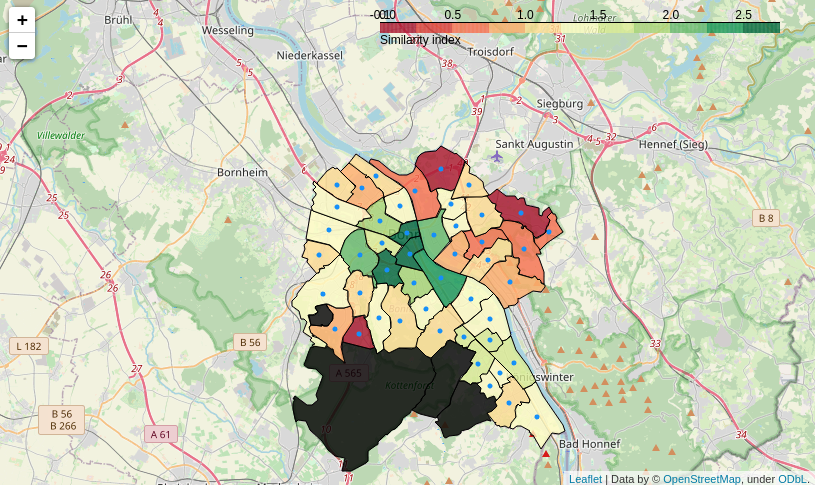
\includegraphics[width=\linewidth]{Figs/Map_similarity_Neighborhoods}
	\caption{Map, showing Bonn's neighborhoods color-coded by their similarity to Munich. A high similarity index (green) corresponds to a strong resemblance of the neighborhood to Munich, a low similarity index (red) means the neighborhood is very different. Black areas could not be analyzed as they contained no venues listed on Foursquare.}
	\label{fig:map_similarity}
\end{figure}

\section{Determination of most similar neighborhood cluster}

Figure~\ref{fig: clusters} shows the five neighborhood clusters we have found in Bonn. The clustering shows that neighborhoods bordering the Rhine are predominantly grouped in the same cluster. Three of the clusters contain only a single neighborhood. This finding could mean that these three neighborhoods have unique characteristics that distinguish them from the rest of Bonn.

\begin{figure}
	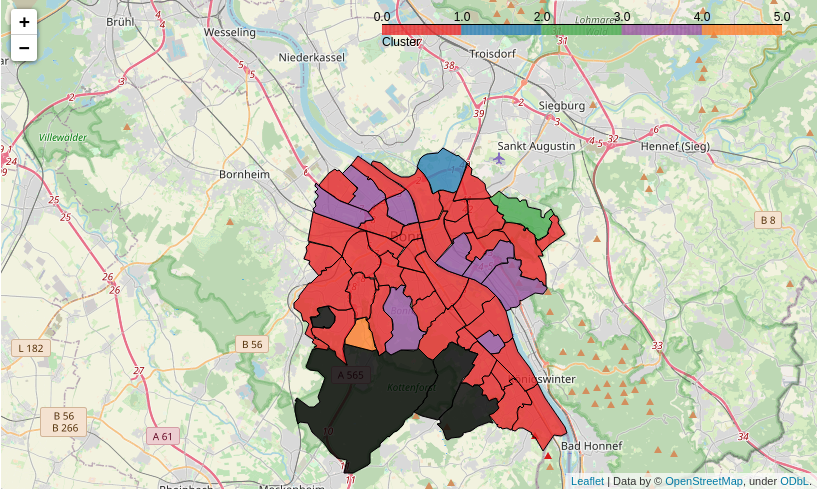
\includegraphics[width=\linewidth]{Figs/Map_clusters}
	\caption{Neighborhood clusters in Bonn. Neighborhoods in the same cluster are colored the same. Black areas could not be analyzed as they contain no venues listed on Foursquare}
	\label{fig:clusters}
\end{figure}

The similarity index of each cluster to Munich is given in Table~\ref{tab: clusters}. We see that the cluster containing the areas at the Rhine is most similar to Munich. This cluster includes the neighborhoods we identified as most similar to Munich in the previous analysis (\emph{Südstadt, Bonn-Zentrum} and \emph{Poppelsdorf}), so this result fits the previous analyses.

\begin{table}
	\caption{Neighborhood clusters in Bonn, their dissimilarity and their similarity to Munich}
	\label{tab:clusters}
	\begin{tabular}{lp{5cm}rr}
		\toprule
		Cluster label &                                                                                                                                                                                                                                                                                                                                                                                                                                                                    Neighborhoods &  Dissimiliarity to Munich &  Similarity to Munich \\
		\midrule
		0             &  Bonn-Zentrum, Buschdorf, Dottendorf, Dransdorf, Endenich, Graurheindorf, Gronau, Ippendorf, Kessenich, Lessenich/Meßdorf, Nordstadt, Poppelsdorf, Südstadt, Weststadt, Alt-Godesberg, Friesdorf, Godesberg-Nord, Hochkreuz, Lannesdorf, Mehlem, Muffendorf, Pennenfeld, Plittersdorf, Rüngsdorf, Beuel-Mitte, Beuel-Ost, Hoholz, Holtorf, Küdinghoven, Pützchen/Bechlinghoven, Schwarzrheindorf / Vilich-Rheindorf, Vilich, Vilich- Müldorf, Brüser Berg, Duisdorf, Lengsdorf &                  0.004071 &               2.390279 \\
		3             &                                                                                                                                                                                                                                                                                                                                                                     Auerberg, Bonn-Castell, Tannenbusch, Venusberg, Godesberg-Villenviertel, Limperich, Oberkassel, Ramersdorf &                  0.010488 &               1.979308 \\
		1             &                                                                                                                                                                                                                                                                                                                                                                                                                                                                       Geislar &                  1.128538 &              -0.052516 \\
		2             &                                                                                                                                                                                                                                                                                                                                                                                                                                                                       Holzlar &                  1.128538 &              -0.052516 \\
		4             &                                                                                                                                                                                                                                                                                                                                                                                                                                                                     Ückesdorf &                  1.128538 &              -0.052516 \\
		\bottomrule
	\end{tabular}
\end{table}


\chapter{Discussion}
\label{sec:Discussion}
All three parts of our analysis give similar results. Both the qualitative analysis in Sect Ref and the quantitative ranking of neighborhoods in Sect REF identify \enquote{Südstadt}, \enquote{Bonn-Zentrum} and \enquote{Poppelsdorf} as highly similar neighborhoods to the Munich area. All three of these neighborhoods are also part of the neighbour hood cluster most similar to Munich.  We conclude that they are the most similar to the Munich area.

In all three analyses, \emph{Ückesdorf} and \emph{Küdingshoven} were identified as very dissimilar to Munich. They do not share any of the top three venue categories with Munich, they have high dissimilarity indices, and they are not part of the neighborhood cluster most similar to Munich.

We have also found an interesting trend. Neighborhoods close to the Rhine resemble Munich much more than neighborhoods away from the Rhine. We infer that the area close to the river marks Bonn's more urban part, which is more similar to the metropolis Munich. Areas away from the Rhine are more suburban or rural and consequently less like Munich.

There are two limitations to our analysis. First, we could not analyze four of the 51 neighborhoods. These neighborhoods had no venues listed on Foursquare. Our study is therefore inconclusive as to whether these neighborhoods are similar or dissimilar to the Munich area. 

Second, the k-means clustering algorithm is sensitive to the choice of $k$. While we justified our choice by estimating the "elbow" in the inertia-$k$ plot for our data, this choice remains arbitrary. A different $k$ leads inevitably to different clusters, and therefore, other neighborhoods might join the cluster most similar to the Munich area. However, we found, that for all $k$ between 2 and 10, the neighborhoods \emph{Südstadt}, \emph{Bonn-Zentrum} and \emph{Poppelsdorf} remain part of the closest cluster.

Based on our results, we give the following recommendations:
\begin{itemize}
	\item We recommend a move to \emph{Südstadt}, as this neighborhood has the highest similarity index to the Munich area.
	\item Viable alternatives are the areas \emph{Bonn-Zentrum} and \emph{Poppelsdorf}, which also have high similarity indices.
	\item We recommend not moving to \emph{Ückesdorf}, \emph{Holzlar} or \emph{Geislar}, as these neighborhoods are very dissimilar from the Munich area.
\end{itemize}


\chapter{Conclusion}
\label{sec:Conclusion}
\section{Summary}
In this report, we analyzed which neighborhood in Bonn is closest to a specific area in Munich. This question is relevant for anyone considering a move from Munich to Bonn. We explored this question with data on the location and category of venues from Foursquare and publicly available location data from the city administration of Bonn. Using this data, we ranked each neighborhood in Bonn according to their similarity to Munich in their occurrence of venues of specific categories. We also grouped similar neighborhoods in Bonn using the k-means clustering algorithm and found the neighborhood cluster in Bonn closest to Munich. We find that the neighborhood most similar to the city center of Munich is \emph{Bonn-Zentrum} and that the neighborhoods \emph{Ückesdorf} and \emph{Küdinghoven} are the most dissimilar to Munich. Based on these results, we recommend to {move preferably to Südstadt, Bonn-Zentrum} or Poppelsdorf and to {avoid moving to Ückesdorf, Geislar or Holzlar}.

\section{Directions for future exploration}
One potential avenue to a refined analysis could consist of grouping the venue categories. The dataset considered in this work contains 163 different venue categories, which are treated as mutually exclusive. However, some classes, like "Restaurant" and "French Restaurant", actually overlap. Therefore, it might be worthwhile to group all restaurant-like types to have a more accurate representation of the venues. Another possibility could be grouping the categories "Garden", "Park", and "Nature Preserve".

Another potential improvement to the analysis could be the incorporation of new data. As shown in Sect.~\ref{sec: Data} and discussed in Sect.~\ref{sec: Discussion}, our dataset did not contain any venues in 6 of Bonn's neighborhoods. Finding venues in these areas (for example, with Google maps) to complement our existing dataset could improve the accuracy.

Finally, although we considered a specific Munich address here,  our approach and analyses are fully generalizable to other locations in Munich, Germany, or the whole world. The only limitation is the availability of enough venues listed on Foursquare. However, most regions in the world are accessible with Foursquare. Therefore, we now can analyze the similarity of almost any city in the world compared to Bonn.

\bibliographystyle{myBib} % style aa.bst
\bibliography{biblio} % your references Yourfile.bib
\end{document}